A simulation user in general does not concern themselves with the \ModelDesc.
The integrators are often created during simulation initialization, which
means that the internal data are not accessible to the Trick logging
mechanisms.
The model works behind the scenes, propagating the states of the simulated
vehicles based on the forces and torques acting on the vehicles.

The simulation's dynamics
manager (see \hypermodelref{DYNMANAGER}) directs the
integration of all dynamic bodies registered with it.
Each dynamic body has its state derivatives computed, based on the forces and
torques acting on it.
The \ModelDesc propagates states according to the state derivatives sent
to it. Properly formulating these state derivatives is one of the jobs of the
\hypermodelref{DYNBODY}.

Two of the factors affecting the accuracy of the propagated state are the
choice of the simulation time step, and the algorithm used to numerically
propagate the state. Every integration algorithm has some optimal
time step for a given problem. Running slower than this optimal step
size reduces accuracy because of limitations inherent in the algorithm.
Running faster than this optimal step size degrades accuracy because the
of limitations inherent in the use of IEEE floating point arithmetic.

For spacecraft simulation that include a model of the flight software, the
operation of the flight software often places an upper bound on the simulation
time step.  The flight software time step is often shorter than the optimal
time-step (viewed from the perspective of accurately propagating state),
resulting in a suboptimal choice for integration rates.  Choosing to run
the simulation at a frequency even greater
than the flight software frequency will further degrade accuracy and
performance, while it is not possible to run more slowly than flight software
requires.  In short, changing the simulation time step is often not an
available option.

There is one marked exception to the above discussion. Ofttimes the behavior
of a failed vehicle must be analyzed. As the flight software is not operating
in these scenarios, the flight software time step is not a constraint.
These scenarios can be run at a frequency slower than the flight software
frequency. Doing so will decrease CPU utilization and may well increase
accuracy.

The appropriate choice of the integration algorithm can
enhance accuracy and performance. The burden of selecting the
appropriate compromise between accuracy and performance falls on the
simulation analyst and integrator. To aid in making that decision, a synopsis
of the techniques available in \JEODid\ is presented in
table~\ref{tab:integ_technique_performance}. The second and third columns
specify the number of calls to the integration and derivative class jobs per
simulation time step. The number of times these functions are called is one of
the key factors that determine the amount of CPU time consumed by a simulation.
The last four columns in the table present the three-sigma error bounds on a
circular orbit simulation integrated with $\omega \Delta t = 0.0562^{\circ}$.
For a 400 km LEO orbit, that corresponds to integrating at 1.15 Hz. These error
bounds are depicted graphically in
Figure~\ref{fig:integ_technique_performance}.

\begin{table}[htp]
\centering
\caption{Integration Technique Performance Characteristics}
\label{tab:integ_technique_performance}
\vspace{1ex}
\begin{tabular}{||l|cccccccc|}
\hline
{\bf Technique} &
\tilt{\bf History length} &
\tilt{\bf Stages per cycle} &
\tilt{\bf Accuracy (order)} &
\tilt{\bf Error, 1 orbit} &
\tilt{\bf Error, 3 orbits} &
\tilt{\bf Error, 10 orbits} &
\tilt{\bf Error, 30 orbits} &
\tilt{\bf Error, 100 orbits} \\ \hline \hline
Euler & 0 & 1 & $O(\Delta t)$ &
  400 km & 3000 & 10000 & 10000 & 20000 km \\
Symplectic Euler & 0 & 1 & $O(\Delta t)$ &
  10 km & 10 & 10 & 10 & 10 km \\
RK2 & 0 & 2 & $O(\Delta t^2)$ &
  0.05 km & 0.2 & 0.5 & 2 & 6 km \\
RK4 & 0 & 4 & $O(\Delta t^4)$ &
  0.002 mm & 0.007 & 0.04 & 0.2 & 0.9 mm \\
ABM4 & 4 & 2 & $O(\Delta t^4)$ &
  0.002 mm & 0.006 & 0.03 & 0.2 & 2 mm \\
Beeman's Algorithm & 1 & 2 & $O(\Delta t^2)$ &
  6 m & 20 & 60 & 200 & 600 m \\
\hline
\end{tabular}
\end{table}

\begin{figure}[htp]
\centering
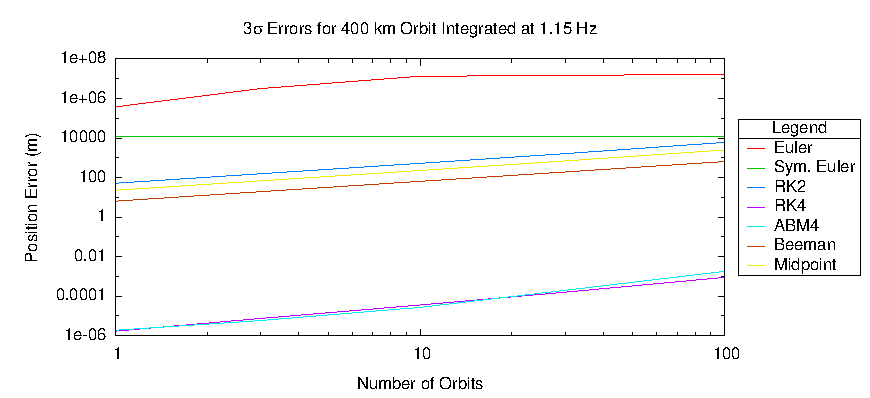
\includegraphics{figures/plot_TranslationTestOrbit_1Hz_monte_err}
\caption{Integration Technique Performance Characteristics}
\label{fig:integ_technique_performance}
\end{figure}


Note that the Euler techniques are quite inaccurate, and their use is
dicouraged.  In particular, use of the basic Euler technique is very strongly
discouraged. It is included with JEOD only because understanding how the basic
Euler technique works is critical for understanding how the more advanced
techniques work.  The symplectic Euler technique may be useful in situations
in which the integration must be
performed at such a high frequency that even a two-stage integrator would be
prohibitively expensive.


\subsection{Changing the Integrator}
The assignment of which integration algorithm will be used is almost always
made at the input file level.  Look for one of the following
specifications:
\begin{verbatim}
 dynamics.manager_init.integ_constructor = trick.<integration-method>()
 dynamics.manager_init.integ_constructor = <sim-object>.<integration-method>
 dynamics.manager_init.jeod_integ_opt = trick.Integration.<integration-method>
 dynamics.manager_init.sim_integ_opt = trick.sim_services.<integration-method>
\end{verbatim}

These are listed in order of preferred practice.

\begin{enumerate}
 \item \textbf{integ\_constructor method with local instantiation}.
 If this method has been used, the
 user will have to look in the S\_define to identify which integrator
 constructors have been included therein.  Look for lines such as

 \verb+##include "utils/integration/include/rk4_integrator_constructor.hh"+

 The integrator can be changed to any of the other integrators for which the
 appropriate header file has been included.  Specifications for
 \verb+<integration-method>+ are:
 \begin{itemize}
  \item ABMIntegratorConstructor
  \item BeemanIntegratorConstructor
  \item EulerIntegratorConstructor
  \item GaussJacksonIntegratorConstructor
  \item RK2IntegratorConstructor
  \item RK4IntegratorConstructor
  \item SymplecticEulerIntegratorConstructor
 \end{itemize}

 Remember to add the () after the specification; this is actually a method
 call to create a new instance of that type of integrator.

 Also be sure to check in the S\_define file to ensure that an instance of the
 IntegratorConstructor has not already been made.  If it has, use option \#2
 (below) instead.

 If the desired integrator is not available, the user may be able to use
 option \#3 (below).


 \item \textbf{integ\_constructor method using S\_define instantiation}.
 If this method has been used,
 the user will have to look in the S\_define to identify which integrator
 constructors have been declared therein (note - these will likely be in the
 simulation object \verb+<sim-object>+).  Any declared constructor can be
 substituted by replacing \verb+<integration-method>+ with the name of
 the instance of another integrator constructor.

 Note that in order for the integrator constructor to be declared, its header
 file must previously be \verb+##include+ in the S\_define, so option \#1
 will, in principle, also work.
 However, if one instance of the integrator
 constructor already exists, another should not be made, so option \#2 is
 preferred \textbf{if} the simulation developer (i.e. the author of the
 S\_define file) has already made such an
 instance.

 If the desired integrator is not available,
 it may be possible to change to option \#3 (below).

 \item \textbf{jeod\_integ\_opt method}. This method can be used with the
 following options for \newline \verb+<integration-method>+:
 \begin{itemize}
  \item Euler
  \item Symplectic Euler
  \item Beeman
  \item RK2
  \item RK4
  \item ABM4
 \end{itemize}
 \item \textbf{sim\_integ\_opt method}.  As a last resort, this method can be
 used with the following options for \verb+<integration-method>+:
 \begin{itemize}
  \item Euler
  \item Euler\_Cromer
  \item Runge\_Kutta\_2
  \item Runge\_Kutta\_4
  \item ABM\_Method
  \end{itemize}
\end{enumerate}

\subsection{Changing the Integration Rate}
The integration rate is typically hard-coded within the simulation.  Look
towards the end of the S\_define file for an entry such as
  \begin{verbatim}
 IntegLoop sim_integ_loop (DYNAMICS) <simulation object list>;
\end{verbatim}
or
\begin{verbatim}
 integrate (DYNAMICS) <simulation object list>;
\end{verbatim}

In either case, the value in parentheses (sometimes a number, sometimes a
parameter) is the integration period.  if a parameter, it will be defined
somewhere in the S\_define, most likely near the top.
\begin{verbatim}
#define DYNAMICS        1.00  // Dynamics interval
\end{verbatim}

There are now two choices for changing the integration rate:
\begin{enumerate}
 \item Change this value; this requires editing the S\_define and recompiling.
 \item Because this value is the simulation-time, and the actual dynamics
 depend on the dynamic-time, it is possible to change (in the input file) the
 actual dynamic-time-step without altering the simulation-time-step by
 altering the rate at which the dynamic-time advances with simulation-time.

 For example,
 \begin{verbatim}
  jeod_time.time_manager.dyn_time.scale_factor = 0.5
 \end{verbatim}
 will make the dynamic-time proceed only half as fast as simulation-time, so a
 simulation-time rate of 1.0 seconds will equate to a dynamic-time rate of 0.5
 seconds.

 Users attempting this change should be familiar with the distinction between
 these two concepts of time. See the \hypermodelref{TIME} for more details.


\end{enumerate}

\subsection{Moving the Integrated Object From One Group to Another}
In rare situation, the simulation may be integrating two different groups of
objects at different rates and.or using different intergators.  It is possible
to switch an object from one group to another, using the
\textit{add\_sim\_object} method.

To identify whether multiple groups are being used, look to the end of the
S\_define for multiple instances of code such as:
\begin{verbatim}
 JeodIntegLoopSimObject <loop_name> (
    <rate>,
    <constructor>,
    <group>,
    <time-manager>,
    <dyn_manager>,
    <gravity_model>,
    <models to be integrated>,
    nullptr);
\end{verbatim}

If this is found, then objects may be moved from one group to another:
\begin{verbatim}
<loop_name>.integ_loop.add_sim_object(<name of object>)
\end{verbatim}
Note - \verb+<loop_name>+ is the name of the group that the object is moving
\textit{to}.


\subsection{Editing the Specifications of the Integrators}
Of the integrators that JEOD provides, only the Gauss-Jackson method has
user-definable specifications.

\subsubsection{Gauss Jackson Parameters}
\label{sec:guide_simuser_gauss_jackson_parameters}
For Gauss-Jackson, the following values can be set:
\begin{itemize}
 \item The order of the integrator.  This defaults to 8, and can be set from 1
 to 16.
 \item The maximum time-step to use on the primer.  This defaults to -1.0;
 indicating that the primer time-step should be the same as the cycle
 time-step and tour time-step.  If the tour time-step is too large for the RK4
 integrator (RK4 serves as the priming integrator, it is used for the first
 few steps) to handle should this value be set.  Set it to a value that is
 appropriate for the limitations of RK4.
 \item Whether or not to perform the convergence test after the correction
 phase.  This defaults to false.
 \item The convergence criterion.  This defaults to $1.0 \times 10^{-9}$.  This
 value is only used if the convergence test is performed.
 \item The maximum number of convergence iterations.  This defaults to 10.  It
 represents the maximum number of times that the state-correction phase can be
 implemented in one integration cycle.  For more precise work, set the
 convergence criterion smaller, and the maximum number of iterations larger.
\end{itemize}

\textbf{Example:}
\begin{verbatim}
 gj_integrator = trick.GaussJacksonIntegratorConstructor()
 gj_integrator.order = 10
 gj_integrator.max_rk4_step= 1.0
 gj_integrator.perform_convergence_test = true
 gj_integrator.convergence_criterion = 1E-10
 gj_integrator.max_corrections_iterations = 15

\end{verbatim}

Note - these values are used in the construction of the integrator.  Once the
constructor has been created, changes to these values will have no effect.
Changes can only be made at the start of the simulation.

The verification simulation \textref{SIM\_GJ\_test}{test:gauss_jackson}
provides a quantitative
illustration of the effect of changing these parameters for a very simple
scenario.

